% SPDX-FileCopyrightText: 2023 SAP SE
%
% SPDX-License-Identifier: Apache-2.0
%
% This file is part of FEDEM - https://openfedem.org

%%%%%%%%%%%%%%%%%%%%%%%%%%%%%%%%%%%%%%%%%%%%%%%%%%%%%%%%%%%%%%%%%%%%%%%%%%%%%%%%
%
% FEDEM Theory Guide.
%
%%%%%%%%%%%%%%%%%%%%%%%%%%%%%%%%%%%%%%%%%%%%%%%%%%%%%%%%%%%%%%%%%%%%%%%%%%%%%%%%

\chapter{Modeling of Joints}
\label{c:Modeling of Joints}

%%%%%%%%%%%%%%%%%%%%%%%%%%%%%%%%%%%%%%%%%%%%%%%%%%%%%%%%%%%%%%%%%%%%%%%%%%%%%%%%
\section{Master and Slave based Joint Modeling}

A joint is a way of specifying a constrained relative motion between two bodies
or links in a mechanism.
In the finite element modeling of mechanism joints, superelement nodes are used
to specify the joint constraints.
A joint between two moving links, denoted 1 and 2, will in general be defined by
one node on link 1, called the slave triad, and one or more nodes on link 2,
called the master triad(s).
The constraints are then modeled by making all DOFs of the slave triad
dependent on all DOFs of the master triad(s), and DOFs of the joint itself.


%%%%%%%%%%%%%%%%%%%%%%%%%%%%%%%%%%%%%%%%%%%%%%%%%%%%%%%%%%%%%%%%%%%%%%%%%%%%%%%%
\section{Single-master Joints}

The position of the slave triad relative to the master triad is given by
%
\begin{equation}
{\mf P}_{SG} \:=\; {\mf P}_{MG}{\mf P}_{JT}{\mf P}_N\cdots{\mf P}_1{\mf P}_{SJ}
\label{eq:JointDef}
\end{equation}
%
where the interpretation of each term is as follows:
%
\begin{namelist}{${\mf P}_{MG}$}

\item[${\mf P}_{SG}$]
Position of Slave triad measured in the Global coordinate system.
The position is ultimately a function of the DOFs of the master triad
and the joint DOFs.

\item[${\mf P}_{MG}$]
Position of Master triad measured in the Global coordinate system.
This matrix is a function of the master triad DOFs and is thus
subject to variation.

\item[${\mf P}_{JT}$]
Position of the Joint measured in the master Triad coordinate system.
This matrix handles a possible offset of the joint relative to the master triad,
as well as joint orientation possibly different from that of the master triad.
The matrix is constant (carries no DOFs) and is thus not subject to variation.

\item[${\mf P}_i$]
Joint variable matrices, numbered from 1 to $N$.
Each matrix can have from 1 to 6 DOFs, or joint variables
(three translations and three rotations).
When all joint variables are zero, each of the matrices ${\mf P}_i$
becomes unity, and \eqnref{eq:JointDef} simplifies to
${\mf P}_{SG} = {\mf P}_{MG}{\mf P}_{JT}{\mf P}_{SJ}$.

\item[${\mf P}_{SJ}$]
Position of the Slave triad measured in the Joint coordinate system,
when all joint variables are zero.
This matrix handles a possible offset of the joint relative to the slave triad,
as well as joint orientation possibly different from that of the slave triad.
This matrix is also constant, and is thus not subject to variation.

\end{namelist}
%
Note that the position of the joint itself, in the global system, is given by
%
\begin{equation}
{\mf P}_{JG} \:=\; {\mf P}_{MG}{\mf P}_{JT}
\label{eq:JointPosGlobSingleMaster}
\end{equation}

The $N$ joint variable matrices ${\mf P}_i$ can be thought of as describing the
relative motion between $N+1$ bodies.
With one single joint variable matrix the two bodies will be the master- and
slave link, respectively (slave link as body 1, and master link as body 2).
With two or more joint variable matrices the intermediate bodies are of course
purely fictitious, although a very useful mental concept.
The joint variables associated with joint variable matrix ${\mf P}_i$ are
expressed in the coordinate system of body $i+1$.
According to~\eqref{eq:JointDef}, this gives the following coordinate system,
$\delta\tilde{\mf u}_1 = {\mf 0}$, for these joint variables:
%
\begin{equation}
{\mf R}_{C_i} =\; {\mf R}_{MG}{\mf R}_{JT}{\mf R}_N\cdots{\mf R}_{i+1}
\quad\text{and}\quad
{\mf R}_{C_N} =\; {\mf R}_{MG}{\mf R}_{JT}
\label{eq:JVarCoordSys}
\end{equation}

Variation of \eqnref{eq:JointDef} provides an expression for the slave DOFs
as a linear combination of the free master DOFs, i.e.
%
\begin{equation}
\label{eq:JointVar}
\eqalign{\delta{\mf P}_{SG} \;
= \;& \delta{\mf P}_{MG}{\mf P}_{JT}{\mf P}_N\cdots{\mf P}_1{\mf P}_{SJ} \cr
+ \;& {\mf P}_{MG}{\mf P}_{JT}\delta{\mf P}_N\cdots{\mf P}_1{\mf P}_{SJ} \cr
\vdots \;& \cr
+ \;& {\mf P}_{MG}{\mf P}_{JT}{\mf P}_N\cdots\delta{\mf P}_1{\mf P}_{SJ} }
\end{equation}
%
since $\delta{\mf P}_{JT}={\mf 0}$ and $\delta{\mf P}_{SJ}={\mf 0}$
according to the definitions above.

The first term of \eqnref{eq:JointVar} provides a linear coupling to the master
triad DOFs, and can be expressed as
%
\begin{equation}
\left[\begin{array}{c}
\delta{\mf u}_s \\
\delta{\tf \omega}_s
\end{array}\right]_M
\;=\;
\left[\begin{array}{cc}
{\mf I} & {\mf \widehat e}_{SM} \\
{\mf 0} & {\mf I}
\end{array}\right]
\left[\begin{array}{c}
\delta{\mf u}_m \\
\delta{\tf \omega}_m
\end{array}\right]
\label{eq:SingleMasterVariation}
\end{equation}
%
where ${\mf e}_{SM}$ is the position of the slave triad relative to the master
triad, measured in global system.
For simplicity, it is here assumed that both the master and slave triad have
DOFs in global directions.

The variation with respect to the joint variables of a given joint variable
matrix ${\mf P}_i$, can be expressed as
%
\begin{equation}
\label{eq:JVarVariation}
\eqalign{
\left[\begin{array}{c}
\delta{\mf u}_s \\
\delta{\tf \omega}_s
\end{array}\right]_i
=\; &
\left[\begin{array}{cc}
{\mf I} & {\mf \widehat e}_{Si} \\
{\mf 0} & {\mf I}
\end{array}\right]
\left[\begin{array}{cc}
{\mf R}_{C_i} & {\mf 0} \\
{\mf 0}       & {\mf R}_{C_i}
\end{array}\right]
\left[\begin{array}{cc}
{\mf 0} & {\mf 0} \\
{\mf 0} & {\mf H}_i
\end{array}\right]
\left[\begin{array}{c}
\delta\tilde{\mf u}_i \\
\delta\tilde{\tf \theta}_i
\end{array}\right] \cr
=\; &
\left[\begin{array}{cc}
{\mf R}_{C_i} & {\mf \widehat e}_{Si}{\mf R}_{C_i}{\mf H}_i \\
{\mf 0}       & {\mf R}_{C_i}{\mf H}_i
\end{array}\right]
\left[\begin{array}{c}
\delta\tilde{\mf u}_i \\
\delta\tilde{\tf \theta}_i
\end{array}\right] }
\end{equation}
%
where ${\mf e}_{Si}$ is the position of the slave triad relative to body $i+1$,
measured in global system.
The matrix ${\mf R}_{C_i}$ defines the coordinate system of joint variable
matrix $i$ according to \eqnref{eq:JVarCoordSys}.
The rotation gradient matrix
${\mf H} = \frac{\partial\tf\omega}{\partial\tf\theta}$
is given by \eqnref{eq:DomegaDtheta}.
Note that in case of only one rotational DOF for joint variable matrix
${\mf P}_i$, this simplifies (in effect) to ${\mf H}_i = {\mf I}$.


\subsection{Revolute Joint}

A revolute joint is modeled from two supernodes located on different links in a
mechanism, see Figure~\ref{fig:RevJoint}.
%
\begin{figure}[b]
\center{
\setlength{\unitlength}{1mm}
\begin{picture}(86,62)(9,4)
\thicklines
% First arm
\qbezier(9,12)(25,35)(37,45)
\qbezier(37,45)(45,50)(51,46)
\qbezier(51,46)(57,42)(52,35)
\qbezier(52,35)(49,30)(36,25)
\qbezier(36,25)(26,19)(17,9)
\qbezier(52,30)(49,25)(36,20)
\qbezier(36,20)(26,14)(17,4)
\qbezier(54.5,41)(54.5,38.5)(54.5,36)
\qbezier(54.5,36)(53.5,32)(52,30)
%
\qbezier(9,12)(13,10.5)(17,9)
\qbezier(17,9)(17,6.5)(17,4)
\qbezier(17,4)(13.5,5.5)(9,7)
\qbezier(9,7)(9,9.5)(9,12)
%Pin
\qbezier(38.5,40)(38.5,43)(43.5,43)
\qbezier(43.5,43)(48.5,43)(48.5,40)
\qbezier(48.5,40)(48.5,37)(43.5,37)
\qbezier(43.5,37)(38.5,37)(38.5,40)
\qbezier(48.5,38.5)(48.5,35.5)(43.5,35.5)
\qbezier(43.5,35.5)(38.5,35.5)(38.5,38.5)
\put(38.6,38.5){\line(0,1){1.5}}
\put(48.6,38.5){\line(0,1){1.5}}
% Second arm
\qbezier(54.2,41)(75,36)(86,23)
\qbezier(44.5,24)(65,23)(80,16)
\qbezier(35.7,19.5)(65,18)(80,11)
%
\qbezier(80,11)(80,13.5)(80,16)
\qbezier(80,16)(83,19.5)(86,23)
\qbezier(86,23)(86,20.5)(86,18)
\qbezier(86,18)(83,14.5)(80,11)
%Z, X0 and Xn vectors
\put(43.5,40){\vector(0,1){13}}
\put(39,50){$Z$}
\put(43.5,55){\vector(0,1){5}}
\put(43.5,55){\vector(0,1){6.5}}
\put(46,56.5){$\tilde\theta_z$}
\put(43.5,40){\vector(-1,-1){10}}
\put(30,26.5){$X_i$}
\put(43.5,40){\vector(2,-1){13}}
\put(57,32){$X_j$}
%\graphpaper[2](0,0)(90,50)
\end{picture}
}
\caption{Coordinate axis and variable of revolute joint.}
\label{fig:RevJoint}
\end{figure}
%
The joint position matrix ${\mf P}_{JT}$ orients the joint coordinate system
to have local $z$-axis along the axis of relative rotation.
The joint has one joint variable matrix with a single DOF, $\tilde\theta_z$:
%
\begin{equation}
{\mf P}_{SG} \:=\; {\mf P}_{MG}{\mf P}_{JT}
{\mf P}_1(\tilde\theta_z)
{\mf P}_{SJ}
\label{eq:RevJointDefault}
\end{equation}
%
Optionally, the joint may also have free motion in the $z$-direction,
in which case it has the additional DOF $\tilde w$:
%
\begin{equation}
{\mf P}_{SG} \:=\; {\mf P}_{MG}{\mf P}_{JT}
{\mf P}_1(\tilde w,\tilde\theta_z)
{\mf P}_{SJ}
\label{eq:RevJointFreeZ}
\end{equation}

The joint produces six constraint equations, one for each slave triad DOF.
Variation of the default revolute joint, \eqnref{eq:RevJointDefault},
will be that of \eqsref{eq:SingleMasterVariation}{eq:JVarVariation}
with the simplifications ${\mf H}_1 = \mf I$, $\delta\tilde{\mf u}_1 = {\mf 0}$,
and $\delta\tilde{\tf\theta}_1 = [0\;0\;\delta\tilde\theta_z]^T$.
With the additional freedom in $z$ as in \eqnref{eq:RevJointFreeZ},
the only change is $\delta\tilde{\mf u}_1 = [0\;0\;\delta\tilde{w}]^T$.


\subsection{Universal Joint}

A universal joint consists of three bodies:
Input Shaft, Center Cross, and Output Shaft.
It is thus modeled with two joint variable matrices to describe the relative
motion between the three bodies (the center cross body is only implicitly
defined through the joint formulation):
%
\begin{equation}
{\mf P}_{SG} \:=\; {\mf P}_{MG}{\mf P}_{JT}
{\mf P}_2(\tilde\theta_z)
{\mf P}_1(\tilde\theta_y)
{\mf P}_{SJ}
\label{eq:UniversalJointDef}
\end{equation}
%
The matrix ${\mf P}_2(\tilde\theta_z)$ here describes the relative motion
(rotation) between the master body and the center cross.
The rotation axis is the $z$-axis of the joint coordinate system.
The matrix ${\mf P}_1(\tilde\theta_y)$ describes the rotation between the
center cross an the slave body.
The rotation axis is here the $y$-axis of the cross coordinate system.
The $y$-axis of the cross coordinate system is initially coincident with
the $y$-axis of the joint coordinate system.
The joint coordinate system will normally be that of the master triad.


\subsection{Constant Velocity Joint}

A constant velocity joint is modeled using the fact that two universal joints
connected via an intermediate shaft will give a constant rotational velocity,
provided that each joint absorbs half of the total angle between the input and
output shaft.
This gives a joint formulation with 4 joint variable matrices,
and two constraint equations that ensure the equal shaft-axis angle between the
two fictitious universal joints:
%
\begin{equation}
{\mf P}_{SG} \:=\; {\mf P}_{MG}{\mf P}_{JT}
{\mf P}_4(\tilde{\theta}_{z_4})
{\mf P}_3(\tilde{\theta}_{y_3})
{\mf P}_2(\tilde{\theta}_{y_2})
{\mf P}_1(\tilde{\theta}_{z_1})
{\mf P}_{SJ}
\label{eq:CVJointDef}
\end{equation}
%
with the additional linear constraint equations
%
\begin{equation}
\tilde{\theta}_{z_4} = \tilde{\theta}_{z_1} \qquad\mbox{and}\qquad
\tilde{\theta}_{y_3} = \tilde{\theta}_{y_2}
\label{eq:CVJointHP}
\end{equation}


\subsection{Ball Joint}

A ball joint is modeled from two supernodes located on different
links in a mechanism, see Figure~\ref{fig:BallJoint}.
The default ball joint formulation has Euler angles $Z-Y-X$ as joint DOFs:
%
\begin{equation}
{\mf P}_{SG} \:=\; {\mf P}_{MG}{\mf P}_{JT}
{\mf P}_3(\tilde\theta_z)
{\mf P}_2(\tilde\theta_y)
{\mf P}_1(\tilde\theta_x)
{\mf P}_{SJ}
\label{eq:BallJoint1}
\end{equation}
%
In addition, the ball joint is available with components of the rotation
axis as joint DOFs:
%
\begin{equation}
{\mf P}_{SG} \:=\; {\mf P}_{MG}{\mf P}_{JT}
{\mf P}_1(\tilde\theta_z,\tilde\theta_y,\tilde\theta_x)
{\mf P}_{SJ}
\label{eq:BallJoint2}
\end{equation}

\begin{figure}[b]
\center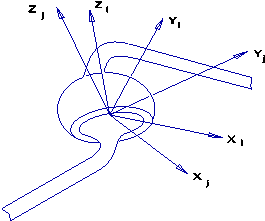
\includegraphics[width=2.8in]{Figures/ballJoint.png}
\caption{Coordinate system i and j of a ball joint}
\label{fig:BallJoint}
\end{figure}

The formulation with the rotation axis parameterization may be used if the
default formulation runs into singularities with respect to the Euler angles.
If singularity arises for the Euler angles, one may also try rotating the joint
(different initial orientation).


\subsection{Rigid Joint}

A rigid joint (see Figure~\ref{fig:RigidJoint}) contains no joint variable
matrices since there is no relative motion between the master and slave bodies.
The joint allows a rigid coupling between two nodes that need not be coincident,
nor is there a limitation on common directions in space:
%
\begin{equation}
{\mf P}_{SG} \:=\; {\mf P}_{MG}{\mf P}_{JT}{\mf P}_{SJ}
\label{eq:RigidJointDef}
\end{equation}

\begin{figure}[t]
\center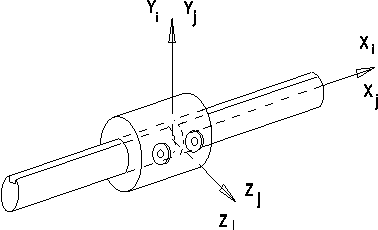
\includegraphics[width=3.9in]{Figures/rigidJoint.png}
\caption{Coordinate axis of rigid joint.}
\label{fig:RigidJoint}
\end{figure}

The rigid joint is often used for accessing internal forces through the
joint at system level during simulation.


\subsection{Free Joint}
\label{subs:Free Joint}

The free joint (see Figure~\ref{fig:FreeJoint}) is modeled from two supernodes
located on ground or different links in a mechanism.
There is full freedom of motion between the links,
provided by six joint variables.
The three translational joint variables are in the coordinate system of the
joint itself, and the three rotational joint variables are Euler angles $Z-Y-X$.
This gives the joint formulation as
%
\begin{equation}
{\mf P}_{SG} \:=\; {\mf P}_{MG}{\mf P}_{JT}
{\mf P}_3(\tilde u,\tilde v,\tilde w,\tilde\theta_z)
{\mf P}_2(\tilde\theta_y)
{\mf P}_1(\tilde\theta_x)
{\mf P}_{SJ}
\label{eq:FreeJoint}
\end{equation}
%
The free joint is also available with components of the rotation
axis as joint DOFs:
%
\begin{equation}
{\mf P}_{SG} \:=\; {\mf P}_{MG}{\mf P}_{JT}
{\mf P}_1(\tilde u,\tilde v,\tilde w,\tilde\theta_z,\tilde\theta_y,\tilde\theta_x)
{\mf P}_{SJ}
\label{eq:FreeJoint2}
\end{equation}

\begin{figure}[t]
\center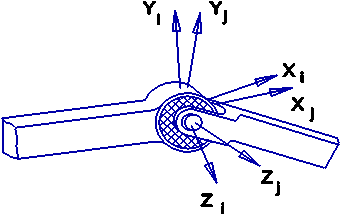
\includegraphics[width=3.55in]{Figures/freeJoint.png}
\caption{Coordinate system i and j for a free joint.}
\label{fig:FreeJoint}
\end{figure}

The reason for having this joint is to facilitate introduction of constraints,
prescribed motions and spring/damper properties on the DOFs represented by the
joint variables rather than the global triad DOFs.
Note that an entirely spring-based free joint formulation, without the joint
variable transformations given by \eqsref{eq:FreeJoint}{eq:FreeJoint2},
also is available for this joint type, see Section~\ref{subs:Global spring}.


\subsection{Axial Joint}

An axial joint is modeled from two supernodes located on two different links.
The joint position matrix ${\mf P}_{JT}$ orients the joint coordinate system
to have its local $x$-axis pointing from the master triad to the slave triad.
The joint has one joint variable matrix with a single DOF, $\tilde u$,
the displacement along the local $x$-axis:
%
\begin{equation}
{\mf P}_{SG} \:=\; {\mf P}_{MG}{\mf P}_{JT}
{\mf P}_1(\tilde u)
{\mf P}_{SJ}
\end{equation}


%%%%%%%%%%%%%%%%%%%%%%%%%%%%%%%%%%%%%%%%%%%%%%%%%%%%%%%%%%%%%%%%%%%%%%%%%%%%%%%%
\section{Multi-master Joints}

The multi-master joints have the same formulation with respect to the relative
motion between the joint itself and the slave triad, as single-master joints.
These joints have an additional variable, called the slider variable $s$,
which expresses the position of the joint (or follower) along a curve defined
by $N$ master triads, i.e, ${\mf P}_{JG}(s)$.
For each master triad, the joint position relative to the triad itself is
defined through ${\mf P}_{JT_i}$, such that the path the follower is to travel
along does not need to go through the triads themselves.
This can be expressed as
%
\begin{equation}
{\mf P}_{JG} \:=\; {\mf P}(s,{\mf P}_{JG_1},\cdots,{\mf P}_{JG_N})
\quad\text{where}\quad{\mf P}_{JG_i} = {\mf P}_{MG_i}{\mf P}_{JT_i}
\label{eq:FollowerFunction}
\end{equation}
%
which resembles the similar expression for the single master joint in
\eqnref{eq:JointPosGlobSingleMaster}.

The variation of \eqnref{eq:FollowerFunction} with respect to the $N$
master triads is
%
\begin{equation}
\left[\begin{array}{c}
\delta{\mf u}_s \\
\delta{\tf \omega}_s
\end{array}\right]_M
\;=\; \sum_{i=1}^N f(s)_i
\left[\begin{array}{cc}
{\mf I} & {\mf \widehat e}_{SM_i} \\
{\mf 0} & {\mf I}
\end{array}\right]
\left[\begin{array}{c}
\delta{\mf u}_{m_i} \\
\delta{\tf \omega}_{m_i}
\end{array}\right]
\end{equation}
%
which closely resembles the similar expression for the single master joints,
\eqnref{eq:SingleMasterVariation}.
If the follower is positioned between node $k$ and $l$,
the interpolation functions $f(s)_i$ will be
%
\begin{equation}
\label{eq:MultimasterWeight}
\eqalign{
f(s)_k \;=\;& (-s-s_l)/(s_l -s_k) \cr
f(s)_l \;=\;& ( s-s_k)/(s_l -s_k) \cr
f(s)_i \;=\;& 0 \quad\mbox{for}\;\; i\ne k \;\;\mbox{and}\;\; i\ne l
}
\end{equation}


\subsection{Prismatic Joint}

The prismatic joint is modeled from three or more supernodes where one node,
the slave triad, is located on the first link while two or more nodes,
the master triads, are located on the second link.
The master triads define a straight line along which the sliding occur,
see Figure~\ref{fig:PrismJoint}.
The slave link can rotate about the $x$- and $y$-axes of the joint,
which gives the following parameterization:
%
\begin{equation}
{\mf P}_{SG} \:=\; {\mf P}_{JG}(s,\cdots)
{\mf P}_2(\tilde\theta_y)
{\mf P}_1(\tilde\theta_x)
{\mf P}_{SJ}
\label{eq:PrismDef}
\end{equation}
%
The $z$-axis of the joint is always pointing in the positive curve direction.

\begin{figure}[b]
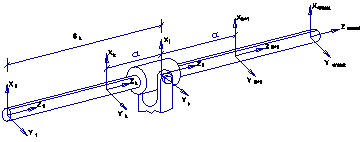
\includegraphics[width=\textwidth]{Figures/prismaticJoint.png}
\caption{Prismatic joint with slave and master nodes.}
\label{fig:PrismJoint}
\end{figure}

To model telescopic motion, two parallel prismatic joints of this type is used
between the same two links of the mechanism.


\subsection{Cylindric Joint}

The cylindric joint closely resembles the prismatic joint, but the slave link
is also free to rotate about the master line itself.
The joint coordinate system has, as for the prismatic joint, the local $z$-axis
along the master curve in positive direction, which gives the parameterization:
%
\begin{equation}
{\mf P}_{SG} \:=\; {\mf P}_{JG}(s,\cdots)
{\mf P}_3(\tilde\theta_z)
{\mf P}_2(\tilde\theta_y)
{\mf P}_1(\tilde\theta_x)
{\mf P}_{SJ}
\label{eq:CylindricDef}
\end{equation}
%
The rotation can also be parameterized using rotation axis components:
%
\begin{equation}
{\mf P}_{SG} \:=\; {\mf P}_{JG}(s,\cdots)
{\mf P}_1(\tilde\theta_z,\tilde\theta_y,\tilde\theta_x)
{\mf P}_{SJ}
\label{eq:CylindricDef2}
\end{equation}


\subsection{Cam Joint}
\label{subs:Cam Joint}

The cam surface is defined by a curve through an ordered set of master triads.
If the first and last master are identical, the cam has a closed surface.
The curve tangent defines the local $z$-axis of the joint coordinate system.
Its local $x$-axis corresponds with the surface normal direction, and is defined
from the local $x$-axis direction of the master triads along the curve.

Currently, the curve defining the cam surface can consist of straight lines
and circle arcs only, each made up of three nodes, see Figure~\ref{fig:Cam}.
A straight line is simply an arc with zero curvature ($1/R\approx0$).

\begin{figure}[t]
\center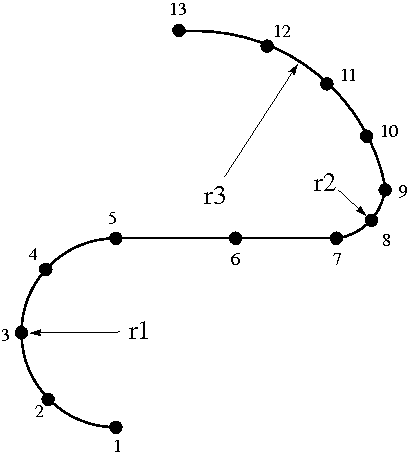
\includegraphics[width=2.2in]{Figures/CamCurve.png}
\caption{Cam curve composed of a circle arc, a straight line, a circle arc
and another circle arc.
The first and last arcs consist of two curve segments (5 nodes).
The straight line and the second arc consist of one curve segment each.}
\label{fig:Cam}
\end{figure}

\remark{It is worth noticing that a sudden change in radii of the curve gives a
discontinuity in the second derivative, resulting in sudden forces in the cam.}

The default master-slave based cam parameterization has full rotational freedom
of the slave link relative to the follower, as well as translational DOFs in
the local $x$- and $y$-direction of the follower, which gives
%
\begin{equation}
{\mf P}_{SG} \:=\; {\mf P}_{JG}(s,\cdots)
{\mf P}_3(\tilde u,\tilde v,\tilde\theta_z)
{\mf P}_2(\tilde\theta_y)
{\mf P}_1(\tilde\theta_x)
{\mf P}_{SJ}
\label{eq:CamDef}
\end{equation}
%
The translational DOFs can be suppressed entirely, and individually,
which give the following three alternative formulations for the cam joint:
%
\begin{eqnarray}
{\mf P}_{SG} &=& {\mf P}_{JG}(s,\cdots)
{\mf P}_3(\tilde u,\tilde\theta_z)
{\mf P}_2(\tilde\theta_y)
{\mf P}_1(\tilde\theta_x)
{\mf P}_{SJ} \label{eq:CamFixY} \\
%
{\mf P}_{SG} &=& {\mf P}_{JG}(s,\cdots)
{\mf P}_3(\tilde v,\tilde\theta_z)
{\mf P}_2(\tilde\theta_y)
{\mf P}_1(\tilde\theta_x)
{\mf P}_{SJ} \label{eq:CamFixX} \\
%
{\mf P}_{SG} &=& {\mf P}_{JG}(s,\cdots)
{\mf P}_3(\tilde\theta_z)
{\mf P}_2(\tilde\theta_y)
{\mf P}_1(\tilde\theta_x)
{\mf P}_{SJ} \label{eq:CamFixBoth}
\end{eqnarray}
%
The rotation can also be parameterized using rotation axis components as for the
ball-, free- and cylindric joints, i.e., instead of \eqnref{eq:CamDef} we have:
%
\begin{equation}
{\mf P}_{SG} \:=\; {\mf P}_{JG}(s,\cdots)
{\mf P}_1(\tilde u,\tilde v,\tilde\theta_z,\tilde\theta_y,\tilde\theta_x)
{\mf P}_{SJ}
\label{eq:CamDef2}
\end{equation}
%
and similarly for~\meqsref{eq:CamFixY}{eq:CamFixBoth}.

% SPDX-FileCopyrightText: 2023 SAP SE
%
% SPDX-License-Identifier: Apache-2.0
%
% This file is part of FEDEM - https://openfedem.org

%%%%%%%%%%%%%%%%%%%%%%%%%%%%%%%%%%%%%%%%%%%%%%%%%%%%%%%%%%%%%%%%%%%%%%%%%%%%%%%%
%
% FEDEM Theory Guide.
%
%%%%%%%%%%%%%%%%%%%%%%%%%%%%%%%%%%%%%%%%%%%%%%%%%%%%%%%%%%%%%%%%%%%%%%%%%%%%%%%%

\subsection{Spring-based cam joint formulation}
\label{subs:Spring-based cam joint formulation}

Contact between the slave triad and the cam surface can be modeled using the
formulation described above in Section~\ref{subs:Cam Joint}, by introducing
non-linear springs in the two translational joint variables $\tilde u$ and
$\tilde v$ of \eqnref{eq:CamDef}, or in one of them only by using
\eqnref{eq:CamFixY} or~\eqref{eq:CamFixX}.
However, in situations with large relative separation between the slave triad
and the cam curve, or if the cam curve has sharp corners (infinite curvature),
the solution might become unstable using this formulation.

A more robust alternative is to use a purely spring-based formulation for such
contact problems\footnote{This spring-based formulation has actually been the
default formulation in Fedem since version R2.5m3.}.
This is actually a multi-master equivalent to the {\em global spring\/}
element described in Section~\ref{subs:Global spring}.
That is, it does not involve a transformation of the free variables according to
\meqsref{eq:CamDef}{eq:CamDef2}.
Instead, the stiffness and force contributions from the springs are added
directly to the slave and (some of) the master triad DOFs of the cam joint.

A set of (up to) six orthogonal joint springs (three translational and three
rotational springs) connect the slave node to the follower location on the
cam curve, i.e., the projection of the slave location onto the cam curve
along the local $x$-direction, see Figure~\ref{fig:CamSpring}.
A spring must always be present in the local $x$-direction
(the surface normal direction), otherwise no contact would be established.
In the other five directions, spring-constraining is optional.
%
\begin{figure}[b]
\begin{center}
\setlength{\unitlength}{1mm}
\begin{picture}(80,50)
\thinlines
\put(0,0){\line(1,0){80}}
\put(0,-3){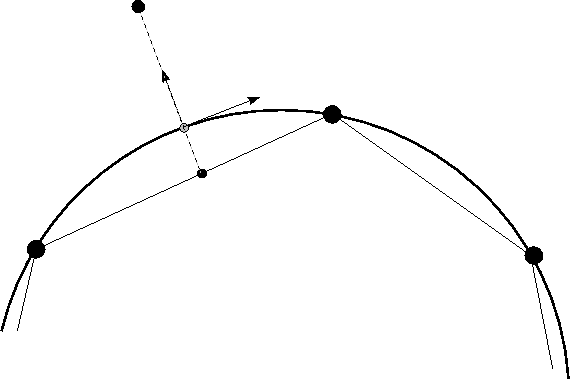
\includegraphics[width=8cm]{Figures/ContactPoint.png}}
\put(22,50){slave node; $S$}
\put(38,36){$z$}
\put(19,38){$x$}
\put(8,13){master node; \large $i$}
\put(45,29){\large $j$}
\put(70,12){\large $k$}
\put(-12,38){contact point; $C$}
\put(14,38){\vector(2,-1){10}}
\put(11,6){master secant point; $M$}
\put(44,10){\vector(-1,1){15}}
\end{picture}
\end{center}
\caption{The geometry of the spring-based cam joint.}
\label{fig:CamSpring}
\end{figure}

\remark{The remark on rotational stiffnesses in global spring elements given in
Section~\ref{subs:Global spring}, also applies to the spring-based cam joint.
Therefore, when using rotational springs, make sure they are stiff enough to
avoid large relative rotations.}

The springs are assumed located at the contact point, $C$, with rigid arms to
the slave node ($S$) and the master secant point ($M$), respectively.
Let ${\mf k}_c = \lceil k_i \rfloor$ and ${\mf f}_c = \{ f_i \}$, $i=1\ldots6$,
denote the diagonal stiffness matrix and the associated force vector of the
compound joint spring in its local system.
The contributions to the slave node are then found as
%
\begin{equation}
{\mf k}_s \;=\; {\mf T}_s{\mf k}_c{\mf T}_s^T \quad\text{and}\quad
{\mf f}_s \;=\; {\mf T}_s{\mf f}_c \quad\text{with}\quad
{\mf T}_s \;=\; \left[\begin{array}{cc}
{\mf I} & {\mf 0} \\ \widehat{\mf e}_s & {\mf I} \end{array}\right]
\end{equation}
%
where ${\mf e}_s = {\mf x}_c - {\mf x}_s$ is the eccentricity vector from the
slave node to the contact point, $C$.
Similarly, the contributions to master node $i$ are found as
%
\begin{equation}
{\mf k}_i \;=\, -f_i(\xi){\mf T}_m{\mf k}_c{\mf T}_m^T \;,\;
{\mf f}_i \;=\, -f_i(\xi){\mf T}_m{\mf f}_c \quad\text{with}\quad
{\mf T}_m \,=\, \left[\begin{array}{cc}
{\mf I} & {\mf 0} \\ \widehat{\mf e}_m & {\mf I} \end{array}\right]
\end{equation}
%
where ${\mf e}_m = {\mf x}_c - {\mf x}_m$ is the eccentricity vector from the
master secant point ($M$) to the contact point, and the function $f_i(\xi)$
is a linear interpolation function distributing the contributions to the two
closest master nodes, and is given by~\eqnref{eq:MultimasterWeight}.

The updated spring lengths in the spring-based cam joint are computed similarly
as for the global spring element of Section~\ref{subs:Global spring}.
However, for the rotational springs we now always assume zero initial angle and
deflection, regardless of the modeling configuration,
such that the computations become
%
\begin{eqnarray}
\label{eq:CamSpringLength}
{\mf l} \;=\hskip4pt \left[\; l_x \hskip6pt l_y \hskip6pt 0\;\right]^T &=&
{\mf R}_c^T({\mf x}_s - {\mf x}_c) \\
\label{eq:CamSpringAngle}
{\tf\alpha} \;=\; \left[\alpha_x \; \alpha_y \; \alpha_z\right]^T &=&
{\rm EulerZYX}({\mf R}_c^T{\mf R}_s^T{\mf R}_{s0}^T{\mf R}_{c0})
\end{eqnarray}
%
Here, ${\mf x}_s$ and ${\mf x}_c$ denote the current global position vectors of
the slave node and the contact point, respectively, whereas ${\mf R}_s$ and
${\mf R}_c$ denote the associated transformation matrices representing their
current orientation, and ${\mf R}_{s0}$ and ${\mf R}_{c0}$
are the corresponding orientations of the initial (modeling) configuration.
It also possible to assign spring properties to the local $z$-direction, and the
spring length $l_z$ is then identical to the current curve length position, $s$.

\subsubsection{Radial contact spring}

By assigning stiffness functions that have zero stiffness in a certain
deflection range around zero, and a high stiffness on both sides outside
this range, it is possible to model that the slave should remain inside
a cylindric surface along the cam curve.
However, for this cylinder to have a circular cross section (like a pipe),
the contact spring(s) should be effective in a radial coordinate system
($r,\theta$), rather than the local Cartesian system ($x,y$).

The polar spring lengths ($l_r,l_\theta$) are obtained from
\eqnref{eq:CamSpringLength} through
%
\begin{equation}
l_r \;=\; \sqrt{l_x^2+l_y^2} \quad\text{and}\quad
l_\theta \;=\; \arctan\left(\frac{l_y}{l_z}\right)
\end{equation}
%
The corresponding spring stiffnesses and forces are then applied in the radial
$r$-direction, and in the circular $\theta$-direction defined such that the
$\theta$-axis is orthogonal to both the $r$- and $z$-directions,
and ($r,\theta,z$) forms a right-handed system.
In addition, we get a geometric stiffness contribution in $\theta$-direction
of magnitude $F_r/l_r$ where $F_r$ is the computed spring force in
$r$-direction, due to the changing direction of the radial spring.

\remark{The radial contact spring must have zero stiffness for small spring
lengths or deflections.
Otherwise, the geometric stiffness term, $F_r/l_r$, will go to infinity
and cause solution instabilities.}



%%%%%%%%%%%%%%%%%%%%%%%%%%%%%%%%%%%%%%%%%%%%%%%%%%%%%%%%%%%%%%%%%%%%%%%%%%%%%%%%
\section{Master and Slave based Transmissions}

Master and slave based transmissions are expressed using linear dependencies
between selected joint variables of the various joint types described above.


\subsection{Gear Joint}

The gear joint is based on two revolute joints, one for the input shaft and one
for the output shaft.
The master triads for these two joints must be placed on the same link---the
gear housing.
Setting the gear ratio to $N$, the linear dependency of the rotational joint
DOFs becomes
%
\begin{equation}
\theta_{z_O} \;=\; N\,\theta_{z_I}
\label{eq:GearConstraint}
\end{equation}
%
where subscript $O$ designates the output shaft, and $I$ the input shaft.


\subsection{Rack and Pinion}

The rack--and--pinion is based on a revolute joint and a prismatic joint.
The master triads of the revolute joint and prismatic joint should be placed
on the same link---the joint housing.
The linear dependency of the rack--and--pinion becomes
%
\begin{equation}
s_O \;=\; N\,\theta_{z_I}
\label{eq:RackAndPinionConstraint}
\end{equation}
%
when using subscript $O$ for the slider variable of the prismatic joint,
and subscript $I$ for the rotational DOF of the input shaft.


\subsection{Screw Joint}

The screw joint is based on a cylindric joint.
The slider DOF is now connected to the rotational DOF about the joint $z$-axis,
which gives the linear dependency
%
\begin{equation}
s_O \;=\; N\,\theta_{z_I}
\label{eq:ScrewJointConstraint}
\end{equation}

% SPDX-FileCopyrightText: 2023 SAP SE
%
% SPDX-License-Identifier: Apache-2.0
%
% This file is part of FEDEM - https://openfedem.org

%%%%%%%%%%%%%%%%%%%%%%%%%%%%%%%%%%%%%%%%%%%%%%%%%%%%%%%%%%%%%%%%%%%%%%%%%%%%%%%%
%
% FEDEM Theory Guide.
%
%%%%%%%%%%%%%%%%%%%%%%%%%%%%%%%%%%%%%%%%%%%%%%%%%%%%%%%%%%%%%%%%%%%%%%%%%%%%%%%%

\section{Joint Friction}

Friction is calculated from forces, moments, and relative velocity in a joint.
The friction properties consist of viscous friction, Coulomb dry friction,
modified Stribeck friction, and friction force caused by prestressed components.
The Stribeck friction yields a continuous description of the friction from
static to sliding movement.

Forces and moments in the joint give an equivalent load, which is the basis for
computing the acting friction force in the joint.
The equivalent load for the various joint types is given in the
Sections~\ref{subs:FricRevJoint}--\ref{subs:FricCamJoint} below.


\subsection{Viscous friction}

Viscous friction can act between any two supernodes or on any joint variable.
The damper force or torque is equal to the damper's viscous coefficient
multiplied by the damper velocity.
%
\begin{equation}
F_{\textit{viscous}} \;=\; c\: V
\end{equation}
%
where $c$ is the damper coefficient.


\subsection{Coulomb friction}

\begin{figure}[b]
\center{
\setlength{\unitlength}{1.2mm}
\begin{picture}(70,40)(-20,-18)
% Axis system
\thinlines
\put(-20,  0){\vector(1,0){60}}
\put(  0,-18){\vector(0,1){38}}
\put( -5,  7){\rotatebox{90}{\textsl{Friction}}}
\put( -1, 21){$F$}
\put( 20, -5){\textsl{Velocity}}
\put( 42, -1){$V$}
%The actual damping function
\thicklines
\put(-20,-10){\line(1,0){20}}
\put(  0,-10){\line(0,1){20}}
\put(  0, 10){\line(1,0){30}}
\put( 32,  9){$F_{\textit{Coulomb}}$}
\end{picture}
}
\caption{Coulomb friction}
\label{figFRIC:Coulomb}
\end{figure}

In classical Coulomb friction models, there is a constant friction force
opposing the motion when the velocity is non-zero. In the case of zero velocity,
the friction opposes all motions as long as the force is smaller in magnitude
than the friction force (see Figure~\ref{figFRIC:Coulomb})
%
\begin{equation}
F_{\textit{Coulomb}} \;=\; \mu_{\textit{Coulomb}}\: F_e\: \text{sgn}(V)
\end{equation}
%
where
%
\begin{namelist}{$\mu_{\textit{Coulomb}}$}
\item[$F_{\textit{Coulomb}}$]   : Coulomb friction force
\item[$\mu_{\textit{Coulomb}}$] : Coefficient of friction
\item[$F_e$]                    : Equivalent normal load
\item[$V$]                      : Velocity
\item[$\text{sgn}(V)$]          : The direction of movement ($\pm 1$)
\end{namelist}

Reduction gears and bearing set-ups are often prestressed to avoid backlash.
This prestress produces friction even when the external load is zero.
This friction component, which is added to the Coulomb friction term.
is defined as (see Figure~\ref{figFric:Prestress}):
%
\begin{equation}
F_{\textit{prestress}} \;=\; F_0\: \text{sgn}(V)
\end{equation}
%
where $F_0$ is the friction force or torque caused by prestressed components
or other constant friction effects.

\begin{figure}[b]
\center{
\setlength{\unitlength}{1.1mm}
%===================== First picture =========================
\begin{picture}(50,45)(-20,-20)
% Axis system
\thinlines
\put(-20,  0){\vector(1,0){45}}
\put(  0,-20){\vector(0,1){40}}
\put( -5, 21){\textsl{Friction}}
\put( 10, -5){\textsl{Velocity}}
\put( 27, -1){$V$}
%The actual friction function
\thicklines
\qbezier[30](-20,-12.5)(-10,-12.5)( 0,-12.5)
\qbezier[30](-20,-10  )(-10,-10  )( 0,-10  )
\qbezier[30](  0, 10  )( 10, 10  )(20, 10  )
\qbezier[30](  0, 12.5)( 10, 12.5)(20, 12.5)
\put(-20,-7.5){\line(1,0){20}}
\put(  0,-7.5){\line(0,1){15}}
\put(  0, 7.5){\line(1,0){20}}
\end{picture}
\hfill
%================== Second picture ==========================
\begin{picture}(50,45)(-20,-20)
% Axis system
\thinlines
\put(-20,  0){\vector(1,0){45}}
\put(  0,-20){\vector(0,1){40}}
\put( -5, 21){\textsl{Friction}}
\put( 10, -5){\textsl{Normal load}}
\put( 27, -1){$F_e$}
\put( -5,  4){$F_0$}
\put(  1, -6){$-F_0$}
%The actual friction function
\thicklines
\qbezier(-20,-9)(-10,-7)( 0,-5)
\qbezier(  0, 5)( 10, 7)(20, 9)
\put(0,-5){\line(0,1){10}}
\end{picture}
}
\caption{Friction caused by prestressed components}
\label{figFric:Prestress}
\end{figure}


\subsection{Modified Stribeck friction}

\begin{figure}[b]
\center{
\setlength{\unitlength}{1.3mm}
\begin{picture}(85,65)(-30,-30)
% Axis system
\thinlines
\put(-30,  0){\vector(1,0){80}}
\put(  0,-30){\vector(0,1){60}}
\put( -5, 32){\textsl{Friction}}
\put( 52, -1){$V$}
%The actual friction function
\thicklines
\qbezier( 0, 20  )(  6, 20)(  8, 16.5)
\qbezier( 8, 16.5)( 10, 13)( 22, 13  )
\qbezier( 0,-20  )( -6,-20)( -8,-16.5)
\qbezier(-8,-16.5)(-10,-13)(-22,-13  )
\put(0, 13){\line( 1,0){38}}
\put(0,-13){\line(-1,0){25}}
\put(0,-20){\line( 0,1){40}}
%
%Equations
\thinlines
\qbezier[30]( 0,20)( 9   ,20  )(18  ,20  )
\put(20  ,19){$F_{\textit{Static}}= (1+S)F_{\textit{Coulomb}}$}
\qbezier[8] (39,13)(41.75,13  )(44.5,13  )
\put(45.5,12){$F_{\textit{Coulomb}}$}
\qbezier[26]( 8,-1)( 8   ,7.75)( 8  ,16.5)
\put( 6.5,-4){$V_{\textit{slip}}$}
%
%Arrows
\thicklines
\put( 0,  6){\vector( 0, 1){3}}
\put( 0,  6){\vector( 0,-1){3}}
\put( 0, 17){\vector( 0, 1){1}}
\put(31, 13){\vector( 1, 0){3}}
\put(31, 13){\vector(-1, 0){3}}
\put( 6, 13){\vector(-1, 0){1}}
\put( 0, -6){\vector( 0, 1){3}}
\put( 0, -6){\vector( 0,-1){3}}
\put( 0,-17){\vector( 0,-1){1}}
\put(-6,-13){\vector( 1, 0){1}}
\put( 7, 18){\vector( 1,-1){1}}
\put(-7,-18){\vector(-1, 1){1}}
\end{picture}
}
\caption{Modified Stribeck friction including hysteresis}
\label{figFric:ModStribeck}
\end{figure}

Modified Stribeck friction defines friction as a constant at extremely low
velocities, then making a smooth transition from higher static friction to the
lower kinetic, or kinetic plus viscous, friction.
A model using modified Stribeck friction predicts a steady motion at extremely
low velocities, instability through a range of velocities, and stable motion
above a certain threshold velocity.

Experiments have verified that after the stiction force has been surmounted,
the friction decreases exponentially reaching approximately 60\% of the
breakaway force. These bends occur at velocities close to zero.
Detailed experiments carried out in industrial manipulators and reduction gears
have confirmed this negative velocity dependence at low velocity.
The hysteresis effect is also added into the Stribeck friction.
It has been observed that the friction curve is not single-valued.
There is a static friction force that is higher than the kinetic friction,
and the friction does not return to the higher static value when the sliding
velocity decreases.
This means that the friction remains at the low Coulomb friction value until
the velocity has changed sign or is zero (see Figure~\ref{figFric:ModStribeck}):
%
\begin{equation}
F_{\textit{Stribeck}} \;=\; F_{\textit{Coulomb}}
(1 + S e^{-(\frac{V}{V_{\textit{slip}}})^2})\: \text{sgn}(V)
\end{equation}
%
where
%
\begin{namelist}{$F_{\textit{Coulomb}}$}
\item[$F_{\textit{Stribeck}}$] : Stick-slip friction as a function of velocity
\item[$F_{\textit{Coulomb}}$]  : Coulomb friction including friction from
                                 prestressed \mbox{\hskip4pt}~components
\item[$S$] : Magnitude of Stribeck effect (stick-slip factor):
\[ S = \frac{F_{\textit{static}}-F_{\textit{Coulomb}}}{F_{\textit{Coulomb}}} \]
\item[$V_{\textit{slip}}$]     : Critical velocity for Stribeck effect
\item[$\text{sgn}(V)$]         : The direction of movement ($\pm 1$)
\end{namelist}


\subsection{Total friction}

The total friction model is a function resulting from the combination of the
three components described above:
%
\begin{equation}
F_{\textit{total}} \;=\; F_{\textit{viscous}} +
\left[ F_0 + \mu_{\textit{Coulomb}} \: F_e
\left( 1 + S e^{-(\frac{V}{V_{\textit{slip}}})^2}
\right)\right]\: \text{sgn}(V)
\end{equation}


\subsection{Equivalent load in revolute joint}
\label{subs:FricRevJoint}

Friction in revolute joints depends on bearing design and joint loads.
The revolute joint transmits the forces $F_x$, $F_y$, and $F_z$ and the bending
moments $M_x$ and $M_y$.
All these forces and moments are carried by the joint bearings.
The first step is to calculate the axial and radial bearing load based on these
joint forces and moments.

\begin{figure}[b]
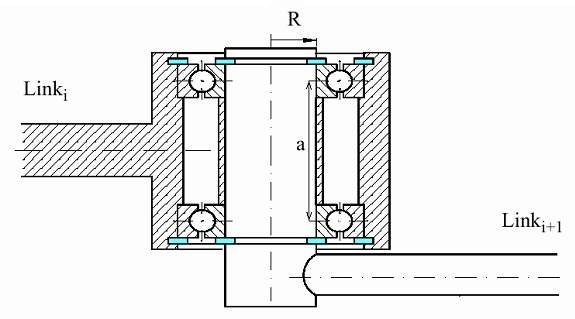
\includegraphics[width=\textwidth]{Figures/FricRevJoint.png}
\caption{Revolute joint}
\label{figFric:RevJoint}
\end{figure}

The revolute joint can be designed and modeled in many ways.
In some cases the joint has only one bearing.
The bending capacity is then calculated by the bearing constant $a$.
This is a standard constant given in bearing catalogs.
If the joint has two bearings as shown in Figure~\ref{figFric:RevJoint},
the joint can also be modeled by using two separate revolute joints,
one at each bearing.
The next step is to calculate the equivalent bearing load as a function of axial
and radial bearing load and bearing geometry. Different types of bearings are
designed to carry either radial or axial load or a combination of these loads.
The equivalent load is then calculated as follows:
%
\begin{eqnarray}
\text{Bearing 1:}\hskip7pt
F_{rx1} &=& \frac{F_x}{2} - \frac{M_y}{a} \nonumber\\
F_{ry1} &=& \frac{F_y}{2} - \frac{M_x}{a} \nonumber\\
F_{r1}  &=& \sqrt{F_{rx1}^2 + F_{ry1}^2} \\[3mm]
%
\text{Bearing 2:}\hskip7pt
F_{rx2} &=& \frac{F_x}{2} + \frac{M_y}{a} \nonumber\\
F_{ry2} &=& \frac{F_y}{2} + \frac{M_x}{a} \nonumber\\
F_{r2}  &=& \sqrt{F_{rx2}^2 + F_{ry2}^2} \\[3mm]
%
\text{Radial bearing load:}\hskip15pt
F_r &=& F_{r1} + F_{r2} \\[1mm]
\text{Axial bearing load:}\hskip15pt
F_a &=& F_z \\[2mm]
%
\text{Equivalent bearing load:}\hskip15pt
\label{eq:BearingLoad}
F_e &=& F_r + F_a Y
\end{eqnarray}
%
where $Y$ is a constant depending on bearing type and geometry, and is
given in the bearing catalogs.
The friction force is calculated as a function of the equivalent bearing load
and the angular velocity. The friction torque in the joint is calculated by
multiplying the friction force by the bearing radius $R$.

A simplified friction representation in revolute joints, where the effects of
the bending moments and the axial load are ignored can also be used.
The coefficients $a$ and $Y$ are then not needed and the equivalent normal
load given by \eqnref{eq:BearingLoad}, reduces to
%
\begin{equation}
\label{eq:RevJointLoad}
F_e \;=\; \sqrt{F_x^2 + F_y^2}
\end{equation}


\subsection{Equivalent load in ball and free joints}

Ball and free joints can both be assigned friction properties to one of its
three rotational DOFs.
The equivalent normal load is then given by \eqnref{eq:RevJointLoad}, where the
indices $x$ and $y$ now represent the two local joint directions that are
orthogonal to the local axis of the chosen friction DOF.
The actual friction torque is then calculated in the same way as for a revolute
joint, based on a specified ball radius $R$ and the angular velocity in the
chosen friction DOF.

For free joints, friction can also be assigned to a translational DOF instead
of a rotational DOF.
The equivalent normal load is then 
%
\begin{equation}
\label{eq:FreeJointLoad}
F_e \;=\; \left\{\eqalign{
F_{e1} = \sqrt{F_y^2 + F_z^2} & \hskip5mm\text{for friction in the Tx DOF} \cr
F_{e2} = \sqrt{F_z^2 + F_x^2} & \hskip5mm\text{for friction in the Ty DOF} \cr
F_{e3} = \sqrt{F_x^2 + F_y^2} & \hskip5mm\text{for friction in the Tz DOF}
}\right.
\end{equation}
%
where $F_x$, $F_y$ and $F_z$ are the joint forces in its local directions.
The actual friction force is then calculated as a function of $F_e$ and
the linear velocity in the chosen friction direction.

\subsection{Equivalent load in prismatic joint}

The friction in a prismatic joint depends on forces normal to the sliding axis
($z$-axis) and forces caused by torque around the $z$-axis.
The joint rotation around the $z$-axis is fixed.
This is usually accomplished by means of a sliding key or similar mechanism
(see Figure~\ref{figFRIC:Prism}).

The friction coefficient in the locking device can in some cases be much higher
than in the linear guidance. This linear bearing is often made of low-friction
rolling elements. Forces in the locking device and normal load in the guidance
are therefore separated and can be weighted by the factor $Y$.
%
\begin{figure}[b]
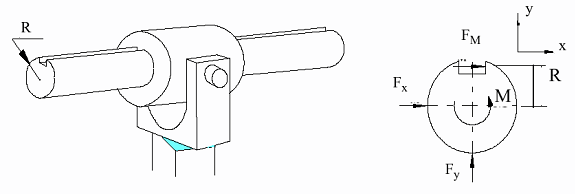
\includegraphics[width=\textwidth]{Figures/FricPriJoint.png}
\caption{Prismatic joint}
\label{figFRIC:Prism}
\end{figure}
%
\begin{eqnarray}
\text{Normal Force:} && F_N \;=\; \sqrt{F_y^2 + (F_x - \frac{M_z}{R})^2} \\
\text{Force in locking device:} && F_M \;=\; \frac{M_z}{R}
\end{eqnarray}
%
Here (see Figure~\ref{figFRIC:Prism}),
$F_y$ and $F_x$ are joint forces in the $y$ and $z$ direction,
$M_z$ is the torque around the sliding $z$-axis, and
$R$ is the radius or distance to the locking device.
The equivalent load is then given by
%
\begin{equation}
\label{eq:PrismLoad}
F_e \;=\; F_N + F_M Y
\end{equation}

A simplified friction representation in prismatic joints, where the effects of
the locking device is ignored can also be used.
The coefficients $R$ and $Y$ are then not needed and the equivalent normal
load, \eqnref{eq:PrismLoad}, reduces to $F_{e3}$ of \eqnref{eq:FreeJointLoad}.

The actual friction force in the prismatic joint is calculated as a function
of the equivalent normal load and the linear velocity of the slider DOF.


\subsection{Equivalent load in cam joint}
\label{subs:FricCamJoint}

The equivalent load in a cam joint is the force between the cam and the follower
in the normal ($x$) direction.
No effect from any translation in the $y$-direction is accounted for.
The equivalent force $F_e$ is thus equal to the force of the contact spring
in the $x$-direction, and the actual friction force is calculated similarly
as for the prismatic joint.

